\chapter{Background Theory, State of the Art and Motivation}\label{T-B}
\label{cha:TheoryAndBackground}
The following chapter elaborates on the background and prestudies for the thesis. It contains a background theory, followed by a literature review and the process of creating the goal of the thesis. Finally the state of the art will be presented and discussed, as well as the motivational foundation of the thesis. 

\section{Background Theory}
The work done in this thesis mainly constitutes two large sub-fields of biological inspired algorithms; namely island models and artificial immune systems. The following section will describe these two fields, as well as covering the concept of classification and genetic algorithms. 

\subsection{Genetic Algorithms}
\label{sec:GA}
Genetic algorithms are a class of iterative search algorithms commonly used in optimisation problems that draws inspiration from biological evolution. Each iteration of the algorithm is referred to as a generation in nature. These algorithms operate on a population of individuals where each individual represent a possible, or parts of a possible, solution to the the problem. One such solution, consisting of a set of genes, is called a chromosome. 

\begin{figure}
    \centering
    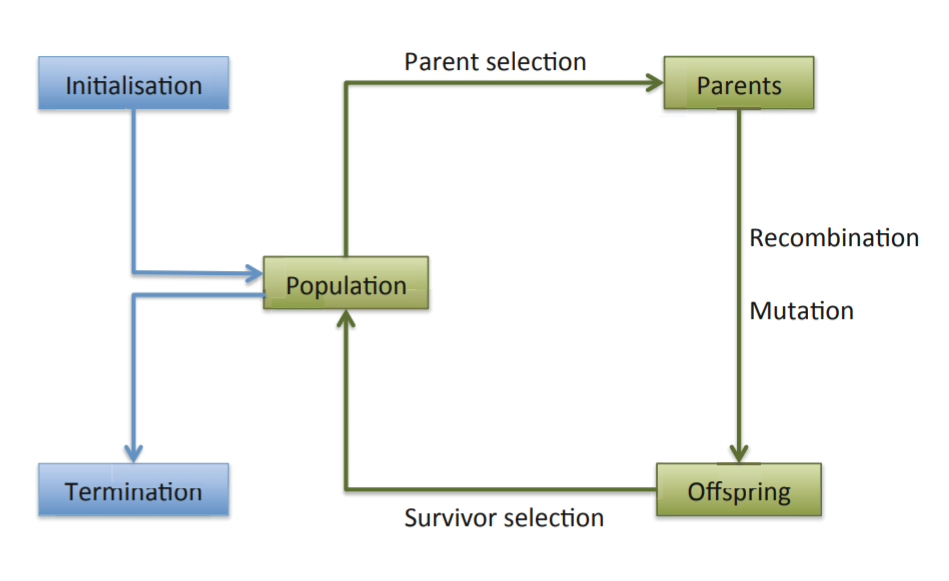
\includegraphics[width=1.0\columnwidth]{figs/GAoverview.PNG}
    \caption[Overview of a genetic algorithm]
    {Overview of a genetic algorithm (adapted from \cite{IntroToEvolutionaryComputing}).}
    \label{fig:GA-overview}
\end{figure}

An example of the processing cycle in a genetic algorithm is presented in figure \ref{fig:GA-overview}. The algorithm starts by creating an initial population of more or less randomly generated individuals. It then uses this initialisation to start its evolutionary cycle, marked as green on the figure. On each iteration individuals are selected for breeding, where stronger individuals have a greater chance of being selected. This selection process is referred to as parent selection, and the breeding process itself is called a crossover, where usually two individuals are combined into one or more offspring solutions. However, the crossover process is not something that is necessarily implemented in a genetic algorithm. The goal here is that while not all newly created individuals need to be stronger than their parents, the population on average should improve over consecutive generations.
%%& not every individual needs to be stronger but across the population you want an improvement. You need we aker individuals too to provide sufficient exploration. 
%%watch words like "trying" to solve.....it is a bit like hopefully etc... 
%% wtach that not all algorithms use crossover. 
The strength of these individuals are calculated as a fitness score based on how well they provide a solution to the problem the algorithm solves. After an offspring has been created there is some chance of parts of the individual being mutated. This can consist of random changes in some of the genes or more informed, heuristic based changes \cite{floreano2008bio}. 

%%watch the discussion about elitism. Such a term is only used when certain individuals are guaranteed to go further. You seem to be using the term elitism to mean two things. Stronger individuals with higher ranking that may have more chance of selection and individuals that are being treated as elite. These two concepts are not the same. 
In addition to parent selection for crossover, genetic algorithms often also employ survivor selection where the fittest individuals are more likely to make it over to the next generation. Therefore, these algorithms strongly apply the principle of survival of the fittest. The number of individuals in a population usually remains constant over the course of the search, meaning that a population size of \textit{n} individuals always makes it to the next round. Typically, you want to prioritise strong individuals over weak when selecting the next generation. However, it is important to not only select the top individuals as this would negatively affect the population diversity. Selecting only the strongest individuals often leads to fast, but premature convergence where the population becomes homogenised, meaning that the population consist of mostly similar individuals. When this happens little to no change is made in the population over successive iterations as the individuals being selected for crossover are all quite similar, and the algorithm typically converges to a local optima. On the other hand, too little prioritisation of strong individuals in the selection process causes the algorithm to diverge, never approaching an exact solution as the algorithm only wanders aimlessly in the search space. Therefore, a careful balance of selecting both strong and weak individuals is required in genetic algorithms to ensure that the fitness of the individuals improves over time at the same time as diversity in the population is maintained \cite{floreano2008bio}.

The process of selection, crossover and mutation are repeated iteratively until the algorithm creates a sufficiently strong individual or the maximum number of iterations is reached. These tasks are often regulated by several parameters, which genetic algorithms tend to have many of. These parameters, which is information passed to the algorithm from the user typically consist of, among others, crossover and mutation rate, maximum iterations and population size. Much of the success of genetic algorithms lies in the choosing and tuning of parameters. 

%Missing diagrams and you may need to think later whether you need to add more details about actual mutation , crossover etc. It depends what the reader needs to know more about to understand your later work.

\subsection{The Island Model}
\label{background:iga}
The island model has become a well known technique for creating genetic algorithms to solve optimisation problems. The technique is usually implemented with \textit{n} sub-populations or islands. Each island runs a genetic algorithm, initialised with its own population and is evolving its population partially isolated from the other islands. The different sub-populations can communicate through the concept of \textbf{migration}. This means that a sub-population can send one or more individuals, to one or multiple sub-populations \cite{IGA:separability_popuplation_size_and_convergence}.
%%as you see here, you are repeating from chapter 1 - removed from chapter 1

In \cite{IGA:DGA-optimization-of-wind-farm} Huang states that there are six important parameters to handle when using IGA. The first is to decide the number of islands or sub-populations and the second would be the population size for each island. I.e, figure \ref{fig:iga:toplogies}(a) illustrates four islands with populations varying from four to six individuals. The third parameter is the island topology, which defines the connection between the islands, also known as the allowed routes for migration from one island to another. As shown in figure \ref{fig:iga:toplogies} three different topologies; (a) is a fully connected topology where the migration routes are available from everyone to everyone, (b) is a star-shaped topology, where one island (the master) have migration routes to all the other islands (slaves), while the slaves only have routes to the master and (c) is a ring-shaped topology, where the migration routes only goes to the island's immediate neighbours. The fourth parameter is the migration rate, which controls how many individuals to migrate from one island to another. The fifth is named migration frequency or migration interval, which defines the frequency of migration. The last parameter is the migration policy, which is the policy for selecting emigrants and the individuals that should be replaced by them. 

\label{fig:island-models}
\begin{figure}
    \centering
    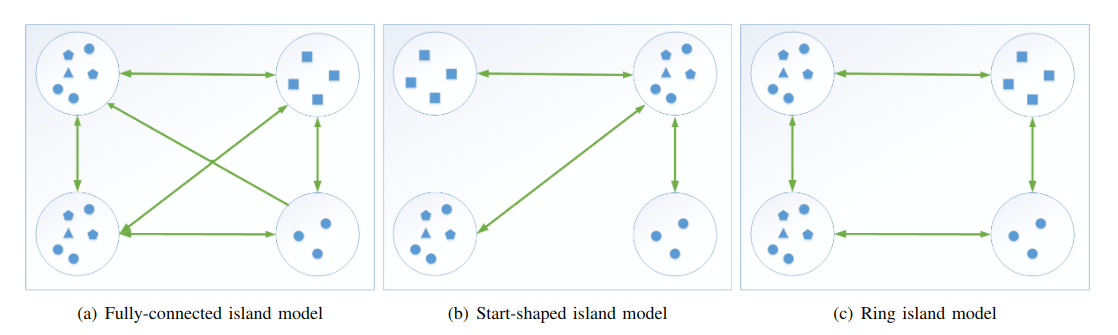
\includegraphics[width=1.0\columnwidth]{figs/island-models.png}
    \caption[Island Topologies]
    {(a) presents a fully-connected island topology (b) presents a star-shaped island topology and (c) presents a ring-shaped topology
    (adapted from \cite{IGA:dynamic_im_based_on_spectral_clustering_in_ga}).}
    \label{fig:iga:toplogies}
\end{figure}

All of the mentioned parameters above are crucial for an IGA, and all of them has an impact on the efficiency and quality of search of the algorithm. Though, another aspect one should take into consideration, especially if the implementation is done in a parallel fashion, is whether the migration should be synchronous or asynchronous. Synchronous migration means that that all all islands migrate their selected individuals at a given time in a generation. Asynchronous migration on the other hand, means that an island can send and receive individuals at any time, or as soon as it find the suited individual(s). Synchronous implementations are usually simpler compared to asynchronous implementations, though the latter are more flexible and efficient \cite{IGA:dea-and-their-models-survey}. 

At last, the choice of homogeneous or heterogeneous islands should be evaluated. In \cite{IGA:dea-and-their-models-survey} Gong at al. describes a homogeneous island model is a model where all islands adopts the same genetic operations, fitness function and selection strategy. This approach is very straight forward, but it some known weaknesses. If the physical layer running the algorithm consists of different processors, the slowest processor will be a bottleneck regarding the efficiency of the algorithm. Also, by letting different subpopulations use the same algorithmic setting, they may not be able to balance local- and global exploration. On the other hand, a heterogeneous island model design can implement different settings or strategies for the different islands, and avoid the weaknesses of a homogeneous design.

%\subsubsection{Migration}
%Migration within IGA allows the sub-populations to share genetic material. This makes it possible for the algorithm to exploit the genetic differences within the different sub-populations. If each island migrate a to large amount of individuals for each generation, a global change of genetic material will occur, which will make the local differences within the islands disappear. Additionally, if the migration happens to rarely, this may lead the small sub-populations to premature convergence \cite{IGA:GA-tutorial-Whitley1994}. 

%need to clarify if the immigrant is the new best individual or what
%also unclear as to whether this happens to just one or all islands in parallel ie synch or unsynch migration

%watch that you have defined what you mean by topology but not structure
% properly planned for a problem...is that realistic...do you not mean that you need to carefully design but you can't know what works...or is there that kind of clarity in research to provide you with such clear rules..

%why advantages and disadvantages here but not above with the GA introduction? 
\subsubsection{Advantages and Disadvantages With the Island Model}
The island model has become a well known and accepted strategy for keeping a high diversity within a population.\cite{IGA:DGA-optimization-of-wind-farm, IGA:dea-and-their-models-survey}
Though, this is not the only benefit one will gain by using the island model. It is known to be very flexible, due two the possibility to have multiple strategies to maintain diversity within the islands. By dividing the population into smaller sub-populations, it will give individuals a better chance for being selected for reproduction, since the mating of individuals only happens within the current sub-population which implies less competition. The offspring of these individuals will also have better chance of being selected for reproduction for the same reasons. The island model may allow weaker individuals to migrate to other populations, as a means of enhancing diversity. Another benefit with this model is that is known for been very efficient \cite{IGA:design-options-impact-effectiveness-and-diversity}; it has an inherent parallel nature, due to the fact that each sub-population is evolving independently. This opens for the possibility of running each island on separate nodes or computers which enables it to exploit such resources effectively. 
%%enhances the computational resources....?? .... requires more resources but may exploit such resources. 

However, the island model also have some drawbacks that needs to be carefully handled. After a certain time of generation, the different islands may start to become quite similar. This can result a loss of diversity within the total population, which is not favourable when trying to find a global optimal solution. Another drawback related to this problem is that maintaining multiple similar, already converged sub-population is a waste of computational resources. Furthermore, when this problem occur, it is hard to determine which islands to maintain and how many that is actually needed \cite{IGA:design-options-impact-effectiveness-and-diversity}.

\subsection{Classification}
Classification is the task of categorising. When this is done by an algorithm it is commonly referred to as machine learning. More formally, machine learning is the process by which the algorithm learns from experience with respect to some class of tasks, and a performance measure to assess how well the assigned tasks perform in the chosen task environment. If the program increases its performance measure at its assigned tasks given its experience, it is said to learn \cite{mitchell1997machine}. Learning is the foundation of machine learning, and subsequently also classification.

Machine learning algorithms can be divided into several types, depending on the problems they solve and how they solve them. Common types include regression, association learning, classification and reinforcement learning. Classification will be the focus of the machine learning aspect of this thesis. As mentioned, classification is the task of categorising, and it is performed given a set of examples with attributes to distinguish, and classes to categorise by. This has many real world applications. An example of this being credit score evaluation in a bank. A bank typically want to assess whether a customer is high or low risk in regards to being able to pay back a loan or not. In other words, the goal is to categorise the customer into one of two different classes; high-risk or low-risk. Each customer is then represented by its set of attributes or \textbf{features}. This set of features could for instance include the customer's age, name, savings, profession and so on. The customer can then be represented in \textit{n}-dimensional feature space, the space containing all possible features of \textit{n} dimensions, where \textit{n} is the number of features assigned to each customer \cite{alpaydin2009introduction}. 

The classification or machine learning task here would then be to find the plane in feature space that best divides the examples into its respective groups. This will usually be done by using a set of pre-labeled training examples; a set of example customer which have already been correctly labelled as one of the two classes. This is also referred to as \textbf{supervised learning} where the algorithm is provided with a set of already classified examples in an attempt create a generalised function and thus also classify new unseen examples, i.e. the task is to best approximate the true function that correctly classifies all examples given a set of already labelled examples. These learned functions takes an input example, also commonly referred to as a case, and returns one or several output classes for that case. Cases used during the supervised learning process is also usually divided into training and test sets. The training set is used to approximate the classification function in the training phase of the algorithm, and the performance of this function is evaluated from seeing how well it is able to generalise when being applied to the unseen cases of the test set \cite{mitchell1997machine}.

\begin{figure}
    \centering
    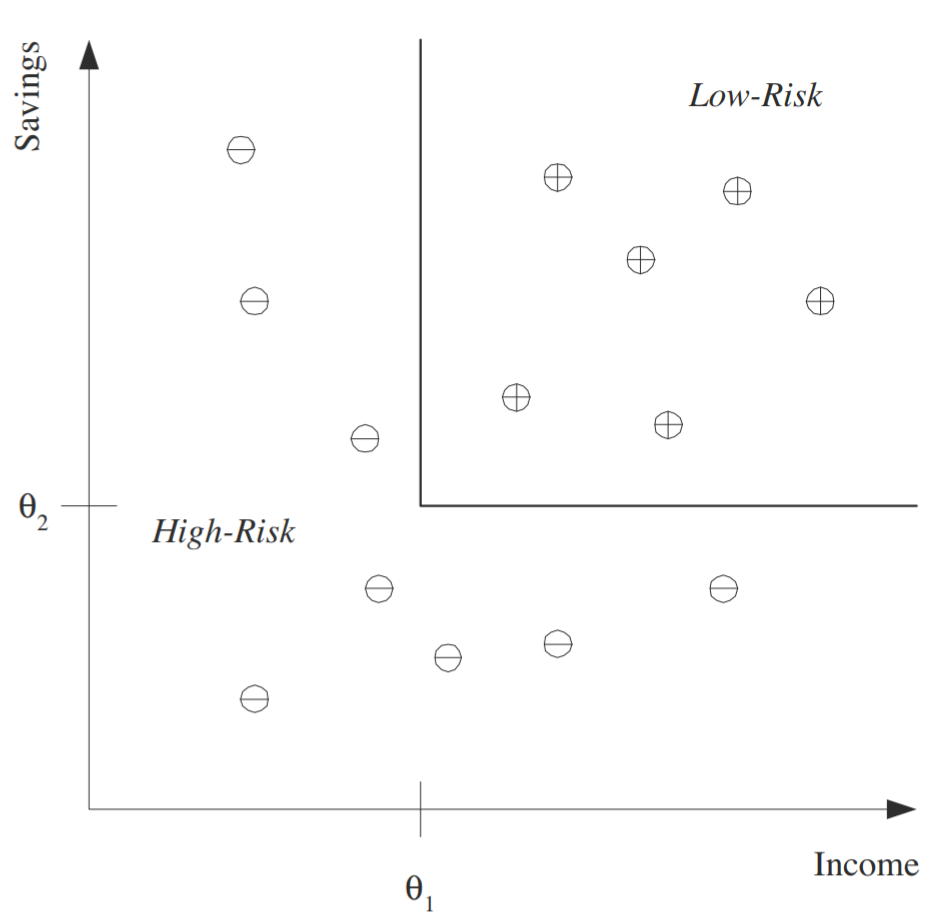
\includegraphics[width=0.5\columnwidth]{figs/machinelearning.PNG}
    \caption[Credit score evaluation problem]
    {Credit score evaluation problem (adapted from \cite{alpaydin2009introduction}).}
    \label{fig:credit-score-evaluation}
\end{figure}

Going back to the credit score evaluation problem one can do a simple representation of each customer by representing them in a 2-dimensional space with only savings and income as features. The classification algorithm could for instance be the process of finding the respective threshold, $\theta_i$, for each feature, and any customer that is above both thresholds (have enough savings and income) is deemed low risk, as shown in figure \ref{fig:credit-score-evaluation}. This can be simplified into a straightforward function such as "IF income is greater than $\theta_1$ AND savings is greater than $\theta_2$ THEN low-risk ELSE high-risk" \cite{alpaydin2009introduction}. Finding this function typically involves several iterations of testing how well the function perform by applying it to the training set, calculating an error value based on its performance and using this error to adjust the function. The algorithm terminates when it correctly classifies all examples, detects premature convergence or reaches the maximum number of allowed iterations \cite{mitchell1997machine}.

This is a very simple function for a simple problem, as in most classification problems the feature space is usually considerably larger. Additionally, the relationships between features will likely a lot be more complex, as well as the algorithm for finding these relationships. However, the key idea to approximate the function that best divides the different cases into its' respective classes remains the same.


\subsection{Immune Systems}
\label{sec:background_ais}
The immune system is arguably one of nature's most highly adaptive, distributed and self-organising systems \cite{AIS:Timmis2004}. It has the property of being able to recognise anomalies; something that deviates from the common rule. This ability to differentiate between organisms that do and do not belong in the body, gives the immune system its inherent classification properties. Through repeated exposure to the same anomalies the immune system is also able to adapt and evolve its cells to combat secondary infections at much higher rates.

\subsubsection{The Natural Immune System}
The natural immune system is the body's natural way of dealing with intruders and otherwise anything that does not fit into the norm. Generally, the immune system is split into two subsections of immunity; namely innate and adaptive immune response. Unlike the adaptive immune system, the innate immune system does not target any specific intruder, but rather anything it deems a pathogen (infectious microorganism) \cite{AIS:Timmis2004}. This innate immune responses is the product of millions of years of evolution and does not change during the lifetime of the host \cite{AIS:janeway2001immunobiology}. Additionally, it works as a controlling organ for the rest of the immune system, and plays a crucial role in administering and triggering immune responses \cite{AIS:Timmis2004}. While the innate immune system is sufficient at protecting the body against microorganisms with certain common molecular patterns it is not able to protect it against anything that hasn't been observed before. Pathogens evolve while the innate immune system does not. 

%watch new terms that are not defined. 
This is why in addition to the innate immune system the adaptive immune system is needed. This part of the immune system has evolved to handle what the innate immune system is not able to recognise. While the innate immune system target any foreign microorganism it is able to recognise, the adaptive system target specific intruders with its variety of immune cells. Furthermore, each cell is able to recognise a certain antigen(foreign substances like toxins and enzymes), or more specifically, the epitope or antigenic determinant, present on the invading microorganism. Upon repeated exposure to such antigen the adaptive immune system is in fact able to adapt and evolve new and specialised antibodies. Antibodies, with paratopes as the antigen-binding site, are the part of the immune cell that is able to recognise and bind to invading antigen \cite{AIS:roitt1994essential}.

The adaptive immune system employs two different types of lymphocytes as immune cells, namely T-cells and B-cells. T-cells functions as the controlling cells of the adaptive immune system, as they initiate the attack, while B-cells are the immune cells that produce antibodies that actually bind to the antigen \cite{AIS:Timmis2004}. 

%%again where are the pics...gets very boring for the reader to see just text... 

\subsubsection{Biological Operations in the Natural Immune System}
As mentioned, upon repeated exposure to new patterns in invading microorganisms the antibodies in the adaptive immune system gradually evolve to recognise these intruders. This is done through a process called affinity maturation. Affinity is a measurement for how well an antibody is able to recognise a specific antigen. Higher affinity means higher strength of the bond between the antibody's epitope and the antigen's paratope \cite{AIS:ClonalSelection}. Figure \ref{fig:antibody-antigen-connection} illustrates how the antibody's paratopes is connected to the antigen's epitopes. The binding strength, and therefore also the affinity between the antigen and the antibody, increases with the amount of connections.  This process occurs during exposure to an antigen, when B-cells with higher affinity are stimulated by the specific antigen to proliferate (divide) with a rate proportional to the corresponding affinity \cite{AIS:AIRS}. This turns the B-cells into either what is called plasma cells, which secrets one type of antibodies, or memory cells that corresponds to what is called immune memory \cite{AIS:Timmis2004}. 

\begin{figure}
    \centering
    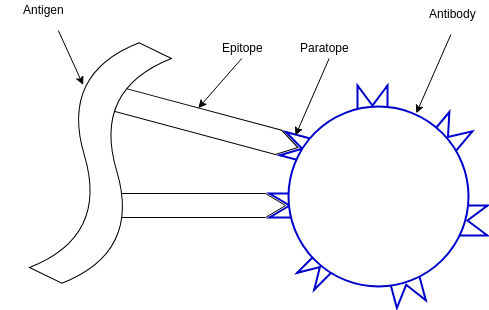
\includegraphics[width=0.8\columnwidth]{figs/antibody-antigen-connection.png}
    \caption{Illustration of an antibody's connection to an antigen}
    \label{fig:antibody-antigen-connection}
\end{figure}

%%somatic hypermutation not defined
During the proliferation process the cloned B-cells are subjected to affinity maturation, which constitutes some somatic hypermuation \cite{AIS:ClonalSelection} along with strong selective pressure that allows the immune system to learn. Somatic hypermutation mutate the variable regions of the antibody genes affecting its capability of binding to certain antigens, which either increase or decrease the affinity of the antibody. During the hypermutation process the B-cells undergo a stochastic alteration of their receptors in an attempt to generate antibodies of higher affinity specialising on the invading antigen. As mentioned above, B-cells of higher affinity are stimulated to proliferate at greater rates, which in turn creates a selective pressure where more capable (higher affinity) B-cells are produced in greater numbers, while lower affinity cells are gradually phased out. Additionally, the mutation process makes the affinity of these cells converge to a point where there are many and capable enough B-cells to combat the current antigen invasion \cite{AIS:Timmis2004}. The theory stating that only the cells being able to recognise the antigen (i.e. cells with greater affinity) proliferate, and therefore being selected over those that do not, is what is referred to as the \textbf{clonal selection principle} \cite{AIS:BackgroundBook}.

%%you haven't said what happens to the B cells that are non memory cells over time
As mentioned, during the proliferation process there is a chance that the B-cell will differentiate into an antibody-secreting plasma cell, or alternatively what is called a memory cell, which is a type of long-lived B-cell that continue to exist in the body even after the antigens and the original B-cells have died. These usually high affinity cells circulate through the body, and when exposed to antigenic stimulus of the same or similar antigen from when they where first created they differentiate into large lymphocytes that produce high affinity cells. This in turn combats the returning antigen at a much higher rate than during the first exposure. These memory cells allow for the immune system to learn and protect against secondary antigen invasions \cite{AIS:Timmis2004}.

%in many ways this seciton is a surprise. Why do you need to talk about algorithmic abstraction here when you don't talke about algorithmic abstraction for the island model or the genetic algorithm. All have algorithmic abstraction. As a reader it makes you think that someone has presented IS in this way so you are..... it is not consistent with the others. You should be interested in abstraction in all parts of your future hybrid models. 
%It seems like you are now matching at least this algorithm to the application. Thing about the flow here. if you are finished introducing the basic concepts of all the algorithm then maybe you are moving to a new section about abstractions where you are matching the background theory to the chosen application. As such it doesn't really belong here. 
\subsubsection{Artificial Immune Systems}
%To create an artificial immune system good abstractions of the core concepts are necessary. This can be done in a number of ways, some which will be presented in the subsequent sections as the more specific abstractions for this project are discussed. However, some important abstractions are necessary for all standard AIS machine learning models. 

Artificial immune systems are algorithms that solve computationally heavy problems by employing immune principles. In such systems one or several immune system components and theories are employed. However, so far no system employ all the principles of the natural immune system and thus there is no algorithm that creates a complete abstraction. The principles used are often those that have elements in common with evolutionary methods, but at the same time exhibit some peculiarities that make them useful for certain applications \cite{floreano2008bio}.

Depending on the principles used and how they are employed a variety of different artificial immune systems with different capabilities and different application areas can be created. Some of these algorithms employ clonal selection and affinity maturation theories as mentioned in the section above, which allow more stimulated antibodies to proliferate at greater rates \cite{floreano2008bio}.  

One basic principle employed in artificial immune systems is the concept of \textbf{shape space}, visualised in figure \ref{fig:shape-space}. Shape space is a common abstraction that allows for the system to interpret the process of antibodies recognising and connecting to antigen in terms of geometric properties of shape and position. The aim of such an abstraction is to simplify the interaction process, at the same time as some similarity to a biological system is kept. In natural immune systems the recognition process is based on the complementarity of the geometric shapes between the surface of the antigens and the antibody receptors, as well as the electric charge distribution on parts of the surface of the detector on the antibody receptor and parts of the antigen \cite{floreano2008bio}.

Mathematically, we can abstract and simplify the representation of this interaction by representing the properties of the antigen and antibody necessary in determining the degree of interaction between them, i.e the binding region of the antibody, as a list on \textit{n} parameters. This list is referred to as the \textbf{generalised shape} of the antibody, stating its position in shape space. What set of values is used to define the generalised shape also determines the complexity of the antibody representation and, subsequently, its interaction with antigens, which in turn is highly dependent on the needs of the AIS model adopted. Using the generalised shape we can place the antibodies, as well as the antigens, as points in the \textit{n}-dimensional shape space, indicated by the black circles and squares in figure \ref{fig:shape-space} \cite{floreano2008bio}. 

%Using the generalised shape of each antibody allows for determining, if any, the degree of interaction between the antibody and all invading antigens when they are represented as different points in \textit{n}-dimensional shape space \cite{floreano2008bio}.

\begin{figure}
    \centering
    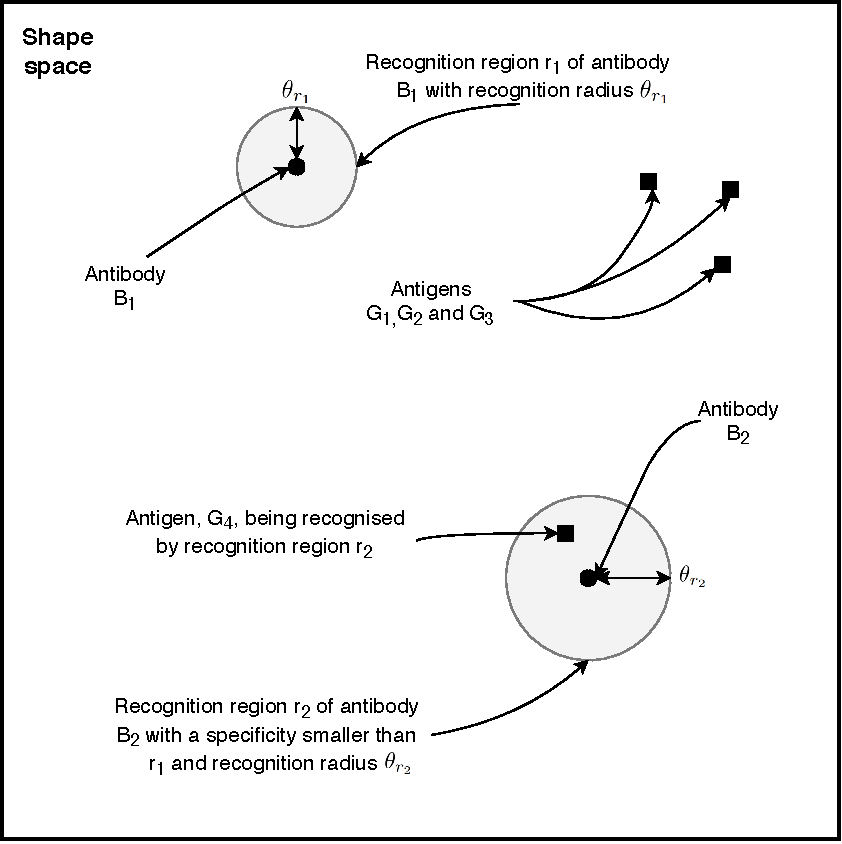
\includegraphics[width=0.7\columnwidth]{figs/ShapeSpace.pdf}
    \caption{Visualisation of the shape space.}
    \label{fig:shape-space}
\end{figure}

However, only representing the antigens and antibodies as points in shape space is not enough for determining the degree of interaction between them. For this we will need to additionally represent how, and under what conditions antibodies recognise antigens. In a natural immune system the degree of interaction or recognition is determined by the complementary of the interacting molecules. However, in an artificial immune system we can ignore the physical properties needed to realise a connection, and simply look at the interaction from an abstract point of view. In such a view we only look at how well the antibodies and antigens match each others' position in shape space, namely to what degree their attributes overlap. In determining the degree of overlap the concept of \textbf{recognition region} is employed. In figure \ref{fig:shape-space} the recognition regions are shown as grey circles surrounding the antibodies. An antibody recognises and connects to all antigens within its recognition region. To determine what is within the recognition region of the antibody a similarity or distance function must be defined. For some antibody, $G_{i}$, and some antigen, $B_{j}$, the distance, and therefore the similarity, between the pair in shape space is defined as the function d($G_{i}$,$B_{j}$). Here, a zero value means a perfect match, and increasingly higher values means decreasingly similar antigen-antibody pairs. Alternatively, a complementary similarity function, s($G_{i}$,$B_{j}$), can be defined to give increasing values to increasingly overlapping antibody-antigen pairs \cite{floreano2008bio}.

Typically, some threshold, $\theta_{r_j}$ is defined for each individual antibody, $B_{j}$, to determine if an antigen, $G_{i}$, is within its recognition region, $r_{j}$, where i=1,2,...,m and j=1,2,...,n. More precisely; if d($G_{i}$,$B_{j}$) $<$ $\theta_{r_j}$ the antigen, $G_{i}$, is said to be within the recognition region of the antibody, $B_{j}$. This is illustrated in figure \ref{fig:shape-space}, where the recognition region of antibody $B_{2}$ contains an antigen, $G_{4}$. Subsequently, when the antigen is within the recognition region of the antibody they are said to be interacting, and the calculated distance between the two can be used in further calculations for determining the affinity between them. In this example, $\theta_{r_j}$ correspond to the radius of a spherical recognition region, where smaller values means a smaller recognition region and therefore a antibody of higher \textit{specificity}, capable of recognising a more specific set of antigens \cite{floreano2008bio}. The concept of specificity is furthermore illustrated in figure \ref{fig:shape-space} where $\theta_{r_2}$ is larger than $\theta_{r_1}$ and therefore less specific. 

What antibodies are connected to what antigens and how well these antibodies solve the problem addressed by the algorithm determines how the antibodies change in order adapt and more correctly recognise as many of the invading antigen as possible. Additionally, the total area covered in the shape space by the unification of the recognition regions of all the different antibodies determines what antigens can be recognised. This area is also what is referred to as the coverage of the \textit{immune repertoire}, here being the set of all antibodies. As there are physical constraints that limit the number of possible configurations for the \textit{n} parameters defining the antigens, the size of the shape space is also consequently finite. Subsequently, a finite number of distinct antibodies with corresponding recognition regions is in theory able to recognise the set of all possible antigens \cite{floreano2008bio}. 

%%was feature space defined earlier? 
%In an artificial immune system the antigen typically correspond to input cases, while antibodies correspond to output classes. Antibodies attempt to predict the class of the antigen. Each antibody is able to recognise one type of antigen, and when it does it binds to said antigen just as in a biological immune system. The strength of the binding between antigen and antibody is determined by how well the attributes of the antigen match the attributes of the antibody. 


%This is usually measured by calculating euclidean (straight-line) distance between the two in feature space. Additionally, to not have to calculate the strength of the connection between every antigen-antibody pair possible, as this would lead to exponential computational costs, the notion of recognition zone is employed. The antibody only binds to antigen within its recognition zone, which is typically defined as a hypersphere of some radius \cite{AIS:Timmis2004}. While hyperspheres are the most common lots of other shapes are possible, shown to give different, and sometimes better results than hyperspheres when certain conditions are met \cite{AIS:NotAllBallsAreRound}.

%%often yeilding.....there is not much research in this area to say that this is a common result.

%Antigen in the artificial immune system are represented as a set of features and therefore as a point in feature space. Additionally, they contain a field for representing their true class, the class the antigen is already pre-labelled with in the data set. The true class is used for accuracy evaluation when comparing the true class to the class assigned by the evolved antibodies. 

%what do you mean by this. A different representation? %%Where have you defined what you mean by the learning process? What is a "true class"

%Antibodies are also represented as a set of features in feature space with a static class selected from the available classes in the classification problem, and the addition of a recognition zone. While antigen remain constant during the course of the algorithm, the antibody population change gradually over successive iterations as their position in feature space and recognition zones are adjusted to provide incrementally better classification accuracies. 

%%this description is a bit unclear. What happens to class?  You have described three elements: set of features, class and recognition zone but only that the set of features and the recognition zone change. 

%%not sure if you have introduced this idea of divide earlier but certainly it is unclear what you mean in this context. What happens to an individ when it divides? What is the difference between the action of divide and the action of cloning. Is cloning not your division without mutation? 

%As the AIS algorithm transition from one generation to the next, antibodies of greater fitness (referred to as affinity in the biological immune system, here meaning stronger connections or more correct classifications) are stimulated to clone itself and mutate in greater numbers than those of lesser fitness. New cells are often created from cloning as in a real biological system \cite{AIS:ClonalSelection}, but since an artificial immune system is in fact artificial it has the ability of increasing or decreasing the biological accuracy depending on the performance of the different mechanics in use. Sometimes completely biologically truthful systems do not yield the best results. Because of this some AIS implement crossover instead of cloning as in \cite{process:valis}. When cloning is used instead of crossover it is increasingly important to use strong mutation operators as there is no crossover operator to produce new and strong combinations of individuals, meaning that the risk of the population becoming homogenised and therefore starting to stagnate increases. Because of this, some AIS algorithms employ a combination of several mutation operators \cite{AIS:elipsis}. 

% if it depends on the biological inspiration then what inspiration leads to the vote. Watch you follow through your statements.... 

%AIS algorithms can operate in several different ways depending on truthfulness of the biological inspiration. One of these ways is to create a system operating in a vote-allocating fashion. Here, a function runs an individual voting process for every antigen, aiming to assign them each a predicted class. Since every antibody contain one of the respective classes of the classification problem it will vote for every antigen it is connected with to belong to its own class.

%%don't think you have actually said this that the class has to be part of the available classes for the classification problem. 
%don't think you have specified that the #antibodies is equal to the number of classes or is it necessarily the case? the wording here would suggest it. 
%%seems to be some mix up with antigens and antibodies here so that this does not make sense. After tidying up the writing I would put in a couple of example pictures to walk the reader through this process to make it clearer. 

%However, vast amounts of antibodies of different classes can be connected to the same antigens, but each antigen can only have one predicted class. Because of this every antigen receives a vote from all its connected antibodies, and the strength of the vote is determined by the strength of the antibody-antigen connection, meaning that votes from antibodies with stronger connection to the antigen have a greater impact on the voting process and therefore the final classification result. When all votes are cast a function counts all the votes given to every class for the antigen, and determines the predicted class of the individual antigen as whatever class has the most votes, which naturally will be the class of one of the connected antibodies. This voting process is done at every iteration of the algorithm, and when all antigen have received a predicted class the accuracy of these predictions are evaluated by comparing them to the known true classes of the antigens. Based on this evaluation the accuracy and performance of the algorithm can be evaluated \cite{process:valis}. Ideally, this will mean that over consecutive iterations, the algorithm will converge towards a fitter population and therefore a population of antibodies increasingly more capable at accurate classifications. Additionally, mutation operators help towards this goal by changing smaller or larger parts of the antibody to increase population diversity and hopefully produce even fitter individuals for the next generation.
%%when all antigens have received a predicted class..... when does this happen? You don't actually state over how or when an antigen actually receives a predicted class. You just talk about voting. at some point you need to see how and when the class info is updated.


%% you suddenly are talking about a single antigen which is in itself confusing. 
%Definitely diagrams are needed that you walk the read through this process rather than this text format. 

\section{Sate of the Art}
\label{sec:no2}
The following section will discuss the challenges and solutions of IGA, followed by a discussion of AIS and its applications and challenges.
\textit{write something else here}
\subsection{The Island Model - Challenges and Solutions}
\label{sec:motivation:iga}
The island model has commonly been used for various optimisation problems such as job shop scheduling problems, feature selection and clustering. The technique has shown promising results on both convergence and quality of outcome. A. L. Corcoran and R. L. Wainwright \cite{IGA:Corcoran} compares different types of genetic algorithms both serial and parallel, including the island model. Their results shows that the serial GA provides good or equal results as the IGA using migration for the smallest problems. Though, compared to the most complex problems, the IGA using migration outperforms the serial GA in both time and quality of result. Antother study presented in \cite{IGA:attribute-reduction} compares three different GAs; serial, IGA without migration and IGA with migration, for attribute reduction. Their results also shows that the IGA with migration outperforms the other two solutions both in time and quality of the result. Such results are due to the parallel nature of IGA. Performance is improved by preserving diversity in the different sub-populations, while the periodic migration makes the quality of selection process  higher \cite{IGA:DGA-optimization-of-wind-farm}. Huang also states in \cite{IGA:DGA-optimization-of-wind-farm} distributed GAs like IGA often is superior (regarding more than just performance) to other serial GAs even when the algorithm runs on a single processor. As a result to this, IGAs is often proven to find the optimal solution faster than a serial GA.

\subsubsection{Number of Islands and Population Size}
The island model has proven to be a successful technique for maintaining diversity in a population. The main reason for this feature is the division of a population into sub-populations. The different sub-population are evolving partially independently which forces them to explore different areas of the search space. How to divide the population into sub-populations and deciding the number of sub-population, can be done in multiple ways. I.e. the islands could be divided into available processors as in \cite{IGA:attribute-reduction}, a dynamic approach like they do in \cite{IGA:dynamic_im_based_on_spectral_clustering_in_ga} or a fixed set of islands based on architectural conditions of the algorithm like in \cite{IGA:Gozali2018}.
S. Areibi at al.  \cite{IGA:advance-iga-for-optimization-problems} presents an IGA for static and dynamic optimisation problems. Their results show clear correlation between the number of islands and quality of the solution, where an increase of islands (and a higher total population) improves the solution. Though, one should note that an increase of islands also increases the computational time of the algorithm. This is mainly because the increase of islands also means an increase of chromosomes in the total population. The implementation of their IGA also follows a ring topology with migration routes going in only one direction. This implies that an increase of islands also will increase the time it takes to share genetic material from $island_1$ to $island_n$. This study also presents results where a fixed population size that is divided across multiple islands, also improves the quality of the solution.

The population size will be one of the IGA parameters that will have an impact on the convergence of the algorithm. It is already known that IGA maintains a relatively high diversity, due to the separate sub-populations which are able to evolve partially on its own. \cite{IGA:dynamic_im_based_on_spectral_clustering_in_ga} Also, in a general GA a large population with high diversity will converge slower, compared with an GA with a small population. This will also yield for the island model. An algorithm where islands have big populations will converge slower than an algorithm with smaller populations \cite{IGA:separability_popuplation_size_and_convergence}. 

\subsubsection{Impact of Island Topology}
As mentioned earlier the island topology defines the allowed migration routes for a chromosomes, or how the different sub-populations are connected. The island topology has a big impact in how the genetic material is shared between the sub-populations, and also have an impact on the isolation level for the different sub-populations. I.e. a ring topology is able to keep a higher isolation over time, than a fully connected topology. This is, of course, because the ring-topology only allows for migration between its two closest neighbouring islands, while the fully-connected topology every island will be allowed to migrate to everyone \cite{IGA:dynamic_im_based_on_spectral_clustering_in_ga}. An overview of the state of the art topologies are presented in figure \ref{fig:island-models}. There exists heaps of other topologies as well, and some are presented in \cite{IGA:survey-of-parallel-DGA,IGA:gong-fukunaga-island-model-random-hetereogeneous-parameter-settings}.

In \cite{IGA:Gozali2018} A. A. Gozali and S. Fujimura presents promesing results with a star-shaped island topology, or a master-slave topology as they refer to it in their research. Three slave islands run three heterogeneous GAs and the master islands has the role of controlling the migration in between the different salve islands. Due to the heterogeneous slave islands, it is implemented with asynchronous migration, controlled by the master island. They manage to keep a high diversity due to their implementation of the master island, which keeps the other islands isolated from each other. In \cite{IGA:DGA-optimization-of-wind-farm} Huang presents a ring topology with one-directional migration routes, with very promising results. This topology is sparsely connected, which means that the chromosomes will spread slower through the different sub-populations than for example in a fully connected topology. This implicitly provides a higher degree of isolation between the sub-populations, which allows different solutions to evolve. These solutions may create better individuals at a later time when they are combined. 

Another approach is a dynamic design presented by Meng at al. in \cite{IGA:dynamic_im_based_on_spectral_clustering_in_ga}. They create an algorithm called DIM-SP (dynamic island model based on spectral clustering), which is initialised with only one island. While evolution proceeds sub-populations migrates to new islands based on similarity between individuals. The central clustering is repeated until the last generation, where all islands are merged together, and the individuals with the highest fitness is considered as the correct solution. Meng at al. also compare DIM-SP to three other IGAs with three different topologies; namely the fully-connected, star-shaped and ring-shaped topologies. DIM-SP finds the best solutions, followed by the ring topology, then the star-shaped topology and at last the fully-connected topology. They find that the ring-topology is in general better than the other star- and fully-connected topology. This is because the ring-model is able to maintain a higher diversity over time, due to its isolating topological features. The other two models show tendencies to converge into the same, due to the dense connections between the islands.

\subsubsection{The Importance of Migration}

As mentioned in section \ref{background:iga}, migration how the different sub-populations in IGA share individuals. It is possible to implement an IGA without migration, though studies shows that IGA without migration does not perform very well \cite{IGA:attribute-reduction, IGA:Corcoran, IGA:DGA-optimization-of-wind-farm}. As the different studies states, this is because the sub-populations tends to converge to fast, and are only capable of finding local optimal solutions. The reason for this is due to relatively small sub-populations that are in full isolation from the remaining population, which will decrease the diversity within the sub-population. 

Despite some poor results without migration, IGA has proven to be very good with migration \cite{IGA:DGA-optimization-of-wind-farm, IGA:attribute-reduction, IGA:Corcoran, IGA:fully-connected-vs-ring-buildings, IGA:non-linear-optimization-problem}. This is because migration is the key for keeping the diversity high within the different sub-populations. Thus IGA exploit the advantage of the rapid convergence with small populations, while also maintaining a high diversity. This often results in an wider exploration of the search space and that higher quality solutions may be found. Though, migration have three important elements that must be handled properly, namely migration rate, migration frequency and migration policy. If the migration- rate and frequency is too high, the sub-population might not be able to evolve in an partially isolated environment. This will eventually lead the sub-populations to migrate into the same, meaning that the diversity within the total population will be lost. Also if the migration- rate and frequency are too low, the different sub-population might converge to fast, due to the lack of diversity. Therefor, both too low or to high migration- rate and frequency can lead to premature convergence, and global optimal solutions might not be found. 

The migration policy is also one of the fundamental elements of migration within IGA. As mentioned in section \ref{background:iga} this defines which individuals to migrate as well as how the new individuals should be integrated in the population. This can be done in multiple ways and one example is presented by Merelo at al. in \cite{IGA:multikulti}. They suggest to migrate multiple individuals, different enough from the receiving population, where the receiving population decides which individuals that should be integrated to promote its own diversity. This policy produces good results, and is proposed as a way to keep the diversity high within the different sub-population, because diversity often lead to exploration of the search space. An other example of a migration policy is presented in  \cite{IGA:gong-fukunaga-island-model-random-hetereogeneous-parameter-settings}. Their migration policy is based on elitism, where the only the best individual is migrated. Migration occurs when a new best individual is found, and is sent to a random neighbouring island. Then the receiving population replaces its worst individual with the new immigrant. Raman at al. in \cite{IGA:attribute-reduction} also presents a similar migration policy, where a percentage of the best individuals are selected for migration, while the receiving population replaces the same percentage of its worst individuals with the new immigrants. Though, migration does not take place ones a new best individual is found, rather after a given time to ensure that the different sub-populations can evolve new good solutions before the next migration. Other studies \cite{IGA:advance-iga-for-optimization-problems, IGA:hybrid-ga-jssp, IGA:DGA-optimization-of-wind-farm} uses some sort of elitism when defining their migration policy. However, as stated in \cite{IGA:DGA-optimization-of-wind-farm}, if each sub-population always sends its best individuals and they replace the worst, this can lead to premature convergence, especially with high migration frequencies. 

%IGA has mostly been used to solve optimisation problems, where performance usually is measured in the computational speed of the algorithm. Though, it has been reported that the technique also provide higher quality solutions than serial GAs \cite{IGA:Corcoran, IGA:attribute-reduction}. 

%above you write about rapid convergence and here you write about avoiding premature convergence. It is not clear what you mean. Just a rewrite needed. 

%\subsubsection{Convergence and Quality}
%The island model has also been proved to not only improve convergence in genetic algorithms, but also the quality in the results. A. L. Corcoran and R. L. Wainwright \cite{IGA:Corcoran} compares different types of genetic algorithms both serial and parallel, where the island model is one of them. Their results shows that the island model with migration does not only provide higher speeds, but also higher quality of the solution. The serial genetic algorithm provides good or equal results for the less complex problems. Though, comparing the hardest problems, one can see that the island model with migration provides higher quality results than any of the other genetic algorithms. M. M. Rahman at al. \cite{IGA:attribute-reduction} presents a study where they compare three different genetic algorithms, serial, island model without migration and island model with migration, for attribute reduction. Their results shows that the island model with migration outperforms the other two solutions both in time and quality of the result. It is also important to mention that the island model without migration often converge to local optimums, due to small population sizes and lack of diversity within the populations. This emphasises once again the importance of the migration policies. Other studies like \cite{IGA:hybrid-ga-jssp,IGA:hybrid-micro-ga} have also compared different implementations of the island model with migration to other genetic algorithms. Both achieve results where the island model with a migration policy outperforms the other genetic algorithms in both time and solution quality. 

\subsubsection{Separable Nature of Problems}
\label{iga:Separable_nature_of_problems}
As mentioned in \cite{IGA:separability_popuplation_size_and_convergence}, the island model has a natural tendency to exploit the separable nature of problems. Linearly separable problems have especially good convergence rates in island model as these are easily separable. Since each island is able to quickly evolve separate parts of the solution to a problem, then merging parts of the islands, a solution to the problem as a whole can quickly be found. Studies also show that it is possible to get linear speedups for non-linear problems, using a distributed genetic algorithm \cite{IGA:non-linear-optimization-problem}.
\todo[inline]{skriv mer om resultatene til den siste kilden.}

\subsubsection{Biological Similarities}
By looking into how evolution works in biology, the famous geneticist Sewall Wright \cite{IGA:wright-inbreeding} argues that having closed populations breed internally with occasional crossbreeding, might greatly improve the convergence rate of the populations. Though, too much inbreeding will lead to extinction and too much mutation will lead to a population of anomalies. If this is compared to the typical island model, one can see that it is based on the same principles. Each island or sub-population is constantly evolving individually, which would be the same as exploiting the rapid convergence of inbreeding. The migration of individuals between the islands will ensure that excessive inbreeding will not take place, and keep a certain diversity in the population. Wright also states that how much inbreeding, mutation and crossbreeding is necessary will vary between the populations and that it is important to maintain a certain balance between the different factors.

One can see that the island model have a lot aspects that are very useful while developing a genetic algorithm. Its core basics is closely related to biological evolution, which is a great incentive for developing genetic algorithms. It allows for running multiple instances of a genetic algorithm at the same time, which is great for separating problems into smaller sub-problems. Additionally, by letting the sub-populations communicate through migration will keep the diversity high which prevents premature convergence. High diversity within the population will lead to a wider search space, which is favourable when trying to find an optimal solution. 


\subsection{Artificial Immune Systems - Applications and Challenges}
\label{sec:motivation_ais}
%%watach that your superlatives are not overstrong.....vast amount...bit over the top... 
Artificial immune systems has gotten attention in various fields in recent years, as it has been shown to have success in a some application areas. These areas include machine learning applications like several supervised learning methods for classification, data clustering and regression. Additionally, AIS has shown great promise within the field of optimisation on, among others, scheduling and multiple objective optimisation problems. 
%% the use of "said" is not correct. Better to drop the word said. there are just certain correct situations and ways to use it in English but the use here is wrong. 
% watch also long sentences
%% don't use "like in". since you are not citing the fact that "most algorithms..." but more giving an example then you would state, for example [x]. However if you were citing the fact that most algorithms... then you would just write []. 
%%high degree of success...needs cite.. 
% watch over use of the word this. in fact try to avoid using this as the reader has to guess what you are referring to...what is this
\subsubsection{Implications of Shape Space}
%Shape space is a term in artificial immune systems that refers to the shape of each receptor. Basically, when abstracting the shape space on an algorithmic level, we refer to a \textbf{generalised shape} as all features necessary to categorise the binding region of the antibody. The generalised shape can in turn be represented by a feature vector made from its necessary attributes, of length \textit{n}, in an \textit{n}-dimensional space, termed the \textbf{shape space} \cite{AIS:Timmis2004}. 
In section \ref{sec:background_ais} the notion of shape space and spherical recognition regions was introduced. However, a spherical recognition region causes some issues as the area covered by hypersheres (spheres of higher dimensionality), and geometric shapes in higher dimensions in general, cover decreasingly less area as the dimensionality of the shape space increases. As dimensions are added to a space, its volume increases exponentially faster, meaning that as dimensionality increases the volume of the hypersphere approaches zero. It is a common problem within machine learning problems, where computation that yields good results in a low-dimensional spaces, becomes intractable in higher dimensions. In fact, it is such a common problem that it is often referred to as a curse, called \textbf{the curse of dimensionality} \cite{AIS:representation-in-ais,AIS:LFS}. 
%%the fact that hypersphere approaches zero is not itself what is referred to as the curse of dimensionality given that not all ML algorithms have the concept of hyperspheres. reword. 
% you also maybe need to have something about fixed size recognition regions and thus fixed sized spheres. 

This means that AIS algorithms may become decreasingly effective when applied to data sets containing a high number of relevant features. Fortunately, some approaches has been proposed to address this problem as in \cite{AIS:representation-in-ais, AIS:LFS}. In  \cite{AIS:LFS} G. Dudek introduces the idea an AIS using \textbf{local feature selection}(LFS). This technique operates on the idea that each component in the algorithm able to classify cases, in this case being the antibodies, consist of a subset of features derived from the complete shape space of the problem. This means that each antibody operate in an specialised \textit{l}-dimensional subspace where \textit{l} is the length of the subset feature vector, and the antibody only considers this feature subset when attempting to classify cases. The use of subspaces subsequently decreases the dimensionality of the problem as most antibodies can then operate on a number of dimensions between 0 and \textit{n} (some antibodies might still have to use the complete shape space of n features). This is illustrated in figure \ref{fig:LFS} where a set of antibodies is first shown to use the whole two-dimensional shape space (a), and another set is shown to all have different sub-spaces of either 1 or 2 dimensions, using different parts of the complete feature space (b).

\begin{figure}[H]
    \centering
    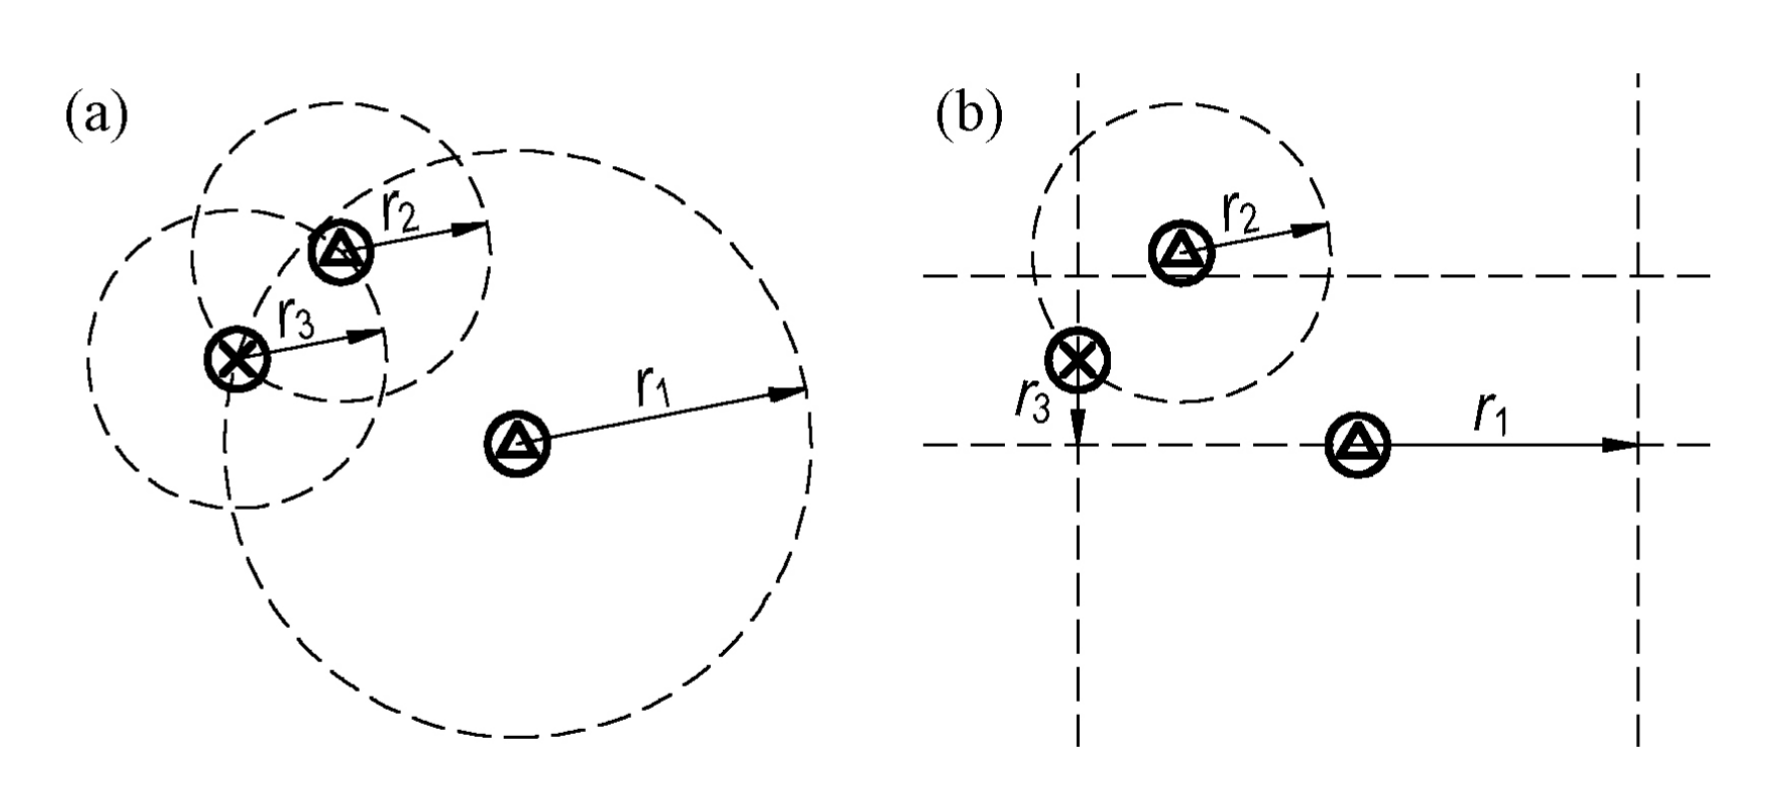
\includegraphics[width=1.0\columnwidth]{figs/LFS.PNG}
    \caption[Local feature selection example]
    {All antibodies (small circles) visualised with their recognition regions (dashed lines) of radius $r_k$ where k = 1,2,3. (a) All antibodies are using the whole 2-dimensional shape space of features \{1,2\}. (b) One antibody of radius $r_2$ using the whole shape space \{1,2\}, another, $r_1$, using just \{1\} and the last one, $r_3$, uses just \{2\} (Adapted from \cite{AIS:LFS}).}
    \label{fig:LFS}
\end{figure}
%%missing pictures to help the understanding

This abstraction is somewhat closer to a real immune system as each derived feature vector represents the specialised receptor of a B-cell as it is. In biology, an arbitrary discontinuous region on a the surface of a molecule, with potentially large differences in area covered between different receptor molecules \cite{AIS:representation-in-ais}. Thus, not representing each antibody as a configuration of all the available features, but rather as a subset of related, but sufficiently different features, creates a biologically closer model. 

Local feature selection is derived from the idea the antibody population of the algorithm is not just a population of centroids, prototypes, or support vectors, but rather a collection of weak learners, each specialising in recognising a certain part of an antigen by its l-dimensional subspace. Each learner or antibody is here a miniature classifier and has, by itself, weak representational capabilities as it is only able to approximate a small part of the total function needed to classify the whole data set. However, when combined in an ensemble-like weighted voting system the population of weak learners together create one strong classifier able to approximate the complete function \cite{AIS:LFS}. 

\subsubsection{Alternative Recognition Regions}

%the description from 9 is fine but it is unclear whether this is the only work or just an example you are using. Would be good to give a clearer understanding of this since your motivation is the state of the art. Who else is thinking this way. If many then you can state something like this and state that you are describing one example. However, if few or the only one then that is important to note too. 
%%watch the use of figures. You have correctly introduced the figure but are not using it. You are assuming that the reader is going to get from the figure what you want him/her to get. However you need to help the reader. As shown.....explanation of what the figure is showing. Look at your cite of [18]. You bring in the cite and then use it to make a point more clearly. Do the same with figures. The idea is the same. Help the reader to understand what part of the figure or citation you want the reader to understand or note. 

\begin{figure}
    \centering
    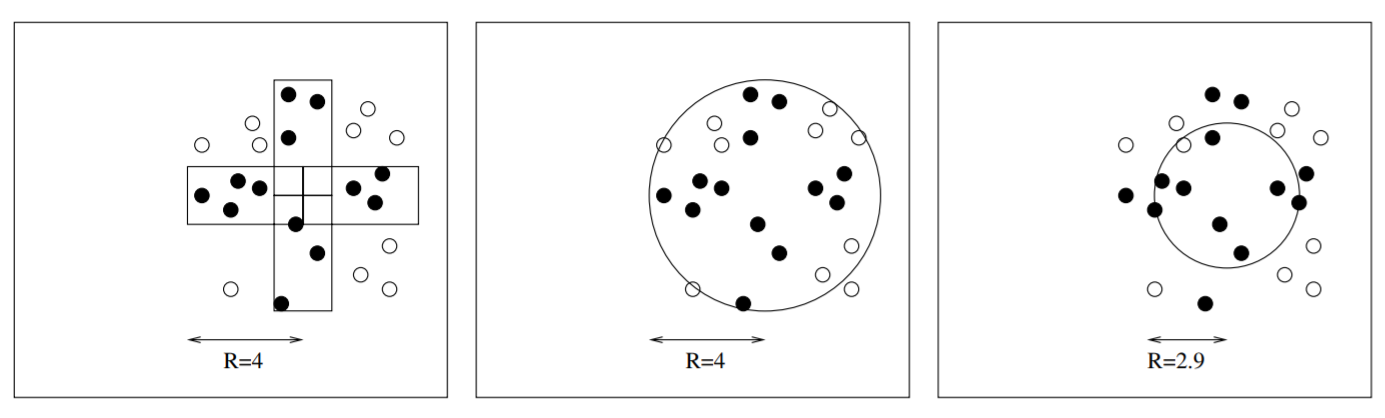
\includegraphics[width=1.0\columnwidth]{figs/reczones.png}
    \caption[Alternative recognition region example]
    {Example of a problem where the choice of recognition region shape is important (adapted from \cite{AIS:NotAllBallsAreRound}).}
    \label{fig:recognition-region}
\end{figure}

As mentioned, section \ref{sec:background_ais} introduced spherical recognition regions. However, several other geometric shapes can be employed for the antibody recognition regions. While hyperspheres are the most commonly used, other shapes have shown to give good results under certain conditions, as a limited number of antibodies of a given shape is not able to correctly classify all data sets. This is illustrated in figure \ref{fig:recognition-region}, where an antibody with a cross-shaped recognition region is able to separate the two classes of data points, while the antibody with a circular region is not. This is especially important when the number of antibodies available to the algorithm is small. This has been shown in \cite{AIS:NotAllBallsAreRound} where they evaluate different recognition zones in a classical AIS, as well as in an idiotypic immune network, where antibodies are able to interact with both antigen and other antibodies. This research display some effects of choosing different recognition region shapes and sizes on the same data, this being that with different recognition regions, networks with different sizes and dynamics are evolved. Additionally, these networks show a varying degree of being able to tolerate antigens given different ranges of recognition radius. Subsequently, the size and shape of the antibody recognition region may affect both accuracy and convergence of the algorithm depending on the parameters and data set used. 


%% I guess you are not emphasising more but rather "more dynamic". I would drop the word more to avoid confusing here. The others are static, as far as i can see. 
Research has been shown to give good results by employing dynamic recognition regions like in \cite{AIS:elipsis} where evolvable elliptical regions have been used. Here, three different mutation operators are used on the recognition regions. These consist of changing the centre of the ellipsis, as well as changing the length and orientation. The resulting algorithm shows no great improvements in regards to solving linearly separable data sets, but on complex nonlinear data sets it appears to perform well and sometimes even better than other algorithms in regards to both training time and accuracy.

\subsubsection{Algorithms}
%%why are you talking about a GA here? . 
%% "as explained in XXX," can shorten this to "see section xx"
How biologically similar one should make an algorithm is always an issue when working with bio-inspired problem solving. There is no definite answer to this and it depends entirely on the methods used and problems solved. This is also naturally true for the field of AIS. While several algorithms have been developed for different optimisation problems it is in the interest of this thesis to look at algorithms applying immune system principles to classification problems, as this is the most relevant application area for this work. 

Generally, in an artificial immune system applied to a classification problem the antigen typically correspond to input cases, while antibodies correspond to output classes. Therefore, antibodies attempt to predict the classes of the antigens. Each antibody is able to recognise one type of antigen, and when it does it binds to said antigen as explained in section \ref{sec:background_ais}. The strength of the binding is typically proportional to the affinity between the interacting antigen-antibody pair. The closer they are to each other in shape space, the better the match is and therefore the resulting affinity will be proportionally high \cite{AIS:Timmis2004}.

Antigen in such an artificial immune system are represented as a set of features and using these as parameters also a point in shape space (See section \ref{sec:background_ais}). Additionally, they contain a field for representing their true class, the class the antigen is already pre-labelled with in the data set. The true class is used for accuracy evaluation when comparing the true class to the class assigned by the evolved antibodies. Antibodies also contains a class label selected from the available classes in the classification problem, and the addition of a recognition zone. While antigen remain constant during the course of the algorithm, the antibody population change gradually over successive iterations as their position in shape space and recognition zones are adjusted to provide incrementally better classification accuracies \cite{AIS:Timmis2004}. 

As the AIS algorithm transition from one generation to the next, antibodies of greater fitness (referred to as affinity in the biological immune system, here meaning stronger connections or more correct classifications) are stimulated to clone itself and mutate in greater numbers than those of lesser fitness. New cells are often created from cloning as in a real biological system \cite{AIS:ClonalSelection}, but since an artificial immune system is in fact artificial it has the ability of increasing or decreasing the biological accuracy depending on the performance of the different mechanics in use. Sometimes completely biologically truthful systems do not yield the best results. Because of this some AIS implement crossover instead of cloning as in \cite{process:valis}. When cloning is used instead of crossover it is increasingly important to use strong mutation operators as there is no crossover operator to produce new and strong combinations of individuals, meaning that the risk of the population becoming homogenised and therefore starting to stagnate increases. Because of this, some AIS algorithms employ a combination of several mutation operators as in \cite{AIS:elipsis}. 

\subsubsection{CLONALG}
One of the most famous AIS algorithms is named CLONALG and is based on the clonal selection and affinity maturation principle used to explain the behaviour of adaptive immune responses in biological immune systems when exposed to antigenic material \cite{AIS:ClonalSelection}. The algorithm is based the established immune system theory of clonal selection, as explained in section \ref{sec:background_ais}, and thus draws strongly from a biological foundation.

\subsubsection{AIRS}
AIRS or Artificial Immune Recognition System is s another famous AIS algorithm. AIRS, as well as CLONALG, is heavily based on the idea that immunological metaphors can be used to create an effective learning algorithm, as it also implements clonal selection and affinity maturation. AIRS follows the shape space model where every receptor has its own fixed position in feature space and bindings between antibody-antigen pairs are calculated as euclidean distances. Additionally, it abandons the immune network model where antibodies can interact with each other. Antibodies are cloned at a rate proportional to the strength of their bindings, with stronger bindings giving a higher degree of stimulation to the antibody. The algorithm employs a fixed population size, so the least stimulated antibodies are continually removed as better performing antibodies emerge from a continuous process of cloning and mutation. These properties has been shown to perform well for classification in a supervised learning system as shown in \cite{AIS:AIRS,AIS:resource-limited-AIS}.

\subsubsection{VALIS}
An AIS algorithm which was recently developed is VALIS; Vote-Allocating Immune System. It operates by allowing all antibodies that contain a given antigen within its recognition region to connect to the antigen, and when connected the class assigned to the antibody is cast as a vote for the antigen. The strength of the connection determines the impact of the vote and the class with the highest count when all votes are summed up is the predicted class of the antigen. This voting process is done at every iteration of the algorithm, and when all antigen have received a predicted class the accuracy of these predictions are evaluated by comparing them to the known true classes of the antigens \cite{process:valis}.

In VALIS if the antigen is within the recognition zone of the antibody the binding weight is 1, otherwise 0. Other AIS algorithms like CLONALG and AIRS does not rely on independent voting based on binding weights as in VALIS, but rather on the most common class of the k-nearest neighbours. VALIS employs, arguably, a more biologically valid method as it relies on local antibody-antigen interactions and not distance-based sorting of antigens as in k-nearest neighbours \cite{process:valis}. On the other hand, VALIS uses a crossover approach when proliferating antibodies, which is in turn less biologically plausible than the cloning process of AIRS and CLONALG.
%%what are you referring to as a standard population model.. is this introduced in an earlier section? If not, perhaps you can say a few words here about the difference. 
%% there are always resource limitation. You never have infinite resources so what are you referring to? 
%%Least stimulated....the reader needs to assume here maybe that stimulation and binding strength are linked or is this something to do with the network?
%% How do Antibodies emerge. It is to grasp the algorithm here. You need to be clearer about what info you need to include to make the point about this algorithm that you want to make and remove all other elements and add what is needed to increase understanding. 

%I am not sure that the class allocation is well explained between here and the earlier section. If two different antibodies have the same Antigen in their recognition regions then what then......they have two different classes.... the strength of the connection between an antigen and an antibody is the overlap of the features but it is unclear what the strength of the connection between the 2 Antibodies with overlapping regions is. I can't find this out ok but you need to clarify this in the text. It is also another issue that the same system is half explained in one place and the rest in another. 
%class distribution of bound antigen for the connected antibody....what is this? 
% make sure every explanation is clear and good. There are many bad explanations in the literature but what you describe in your report needs to be clear. 
% the trade-off is good but seems in the wrong place. Also it is not fully explained. 


\section{Motivation}
Section \ref{sec:no2} elaborates of different aspects of AIS and IGA algorithms, such as challenges, applications and useful techniques. As stated before, the algorithm which will be presented in subsequent chapters attempt to combine these two techniques and their properties. According to the properties discovered through the structured literature review of this thesis certain aspects will be focused. As presented in section \ref{sec:motivation:iga}, IGA has important properties of exploiting the separability of problems, handling large feature spaces, as well as preventing premature convergence. AIS algorithms, on the other hand, have trouble with handling large feature spaces, as discussed in section \ref{sec:motivation_ais}, and like most algorithms employing evolutionary principles, has the risk of suffering from premature convergence (see section \ref{sec:GA}). Through the combination of these techniques we hope to improve on some of the challenges of classification with AIS algorithms. Additionally, the LFS technique, as explained in \ref{sec:motivation_ais}, will be incorporated into the base AIS algorithm and used to further reduce the dimensionality of the shape space, therefore hopefully making the algorithm beneficial to use when applied to complex classification problems with large feature spaces.  

%\subsection{What AIS Properties Could be Enhanced in the Island Model OR Which Properties of AIS Could be Enhanced with/in IGA}

%The problem of evolving a population of weak learners has an inherent separate nature and can be viewed as several smaller problems, which when all solved and working together in an ensemble-like system creates a solution to a larger problem. As discussed in section \ref{iga:Separable_nature_of_problems}, IGA has a tendency to exploit the separability of problems, particularly in linearly separable optimisation problems. However, it is still likely to be useful on other problems, at least when they are complex enough. 
%why is complexity essential for usefulness
%may not help with prediction - have you discussed this earlier, if not then you need to say more or cite someone but preferably give a short explanation. 
%While such an architecture may not help with the prediction task itself, it should at least be favourable in the feature selection part of the algorithm. Letting the different AIS instances divide its' problems on the different islands, it should be possible for all islands combined to generate a complete solution to the problem. Finally, using a technique such as local feature selection to reduce the dimensionality the problems, we believe such an algorithm can improve on both efficiency and accuracy on complex machine learning tasks when compared to other established AIS algorithms.
%am not sure this section belongs here. It has nothing to do with state of the art, more back to your goals. 

